% !TEX program = xelatex
% =====================================================================
%  Slide Beamer: Phát hiện gian lận thẻ tín dụng bằng DBSCAN
%  Biên dịch:  xelatex slide.tex   (mỗi frame = 1 trang, không overlay)
%
%  LƯU Ý "transition mượt":
%   - \transfade (mờ dần giữa các slide) CHỈ phát khi xem bằng Adobe
%     Acrobat / pdfpresenterconsole / Okular. Trình xem thường (Chrome,
%     SumatraPDF) không hỗ trợ transition giữa các slide.
%   - Muốn đổi kiểu transition: \transdissolve, \transwipe, \transpush, ...
% =====================================================================
\documentclass[aspectratio=169,11pt]{beamer}

\usepackage{fontspec}
% Font có đủ ký tự tiếng Việt. Nếu máy không có Segoe UI, đổi sang:
%   \setsansfont{Noto Sans}   hoặc   \setsansfont{Arial}
\setsansfont{Segoe UI}
\setmainfont{Segoe UI}

% ---- Chủ đề & màu (xanh đậm hợp chủ đề tài chính) ----
\usetheme{Madrid}
\usecolortheme{whale}
\setbeamertemplate{navigation symbols}{}

% ---- Transition mượt giữa các slide ----
\newcommand{\mellow}{\transfade[duration=0.5]}

% Bỏ dấu % dòng dưới nếu muốn hiện ghi chú (script) ở màn hình thứ 2 khi trình chiếu:
% \setbeameroption{show notes on second screen=right}

\title{Phát hiện gian lận thẻ tín dụng bằng DBSCAN}
\subtitle{Phương pháp dựa trên mật độ cho bài toán nhãn đến trễ}
\author{[Họ tên --- Mã sinh viên]}
\institute{[Trường / Khoa]}
\date{\today}

\begin{document}

% =====================================================================
% Trang bìa
% =====================================================================
\begin{frame}
  \mellow
  \titlepage
\end{frame}

% =====================================================================
% Slide 1 — Đặt vấn đề & Bài toán
% =====================================================================
\begin{frame}{Thách thức phát hiện gian lận \& Bộ dữ liệu ULB}
  \mellow
  \begin{block}{Thách thức thực tế}
    \begin{itemize}
      \item Nhãn gian lận đến trễ (delayed labels)
      \item Thủ đoạn lừa đảo thay đổi liên tục
    \end{itemize}
  \end{block}
  \begin{block}{Bộ dữ liệu ULB (Kaggle)}
    \begin{itemize}
      \item Tổng giao dịch: \textbf{284.807} dòng
      \item Gian lận thực tế: \textbf{492} giao dịch ($\approx$ 0,17\%)
      \item Đặc trưng: \textbf{30} chiều (28 cột PCA ẩn danh + Time + Amount)
    \end{itemize}
  \end{block}
  \note{"Xin chào thầy cô và các bạn. Bài toán đặt ra là làm sao phát hiện gian lận
  thẻ tín dụng khi dữ liệu nhãn thường đến rất muộn và kẻ gian liên tục đổi thủ đoạn.
  Ở đây chúng tôi dùng bộ dữ liệu kinh điển ULB với gần 285 nghìn giao dịch, nhưng
  tính mất cân bằng cực nặng --- chỉ 492 ca gian lận ẩn trong không gian 30 chiều."}
\end{frame}

% =====================================================================
% Slide 2 — Nhãn đến trễ (Delayed Labels)
% =====================================================================
\begin{frame}{Nhãn đến trễ (Delayed Labels) --- vì sao quan trọng}
  \mellow
  \begin{block}{Khái niệm}
    Trạng thái gian lận thật của giao dịch \textbf{không được biết ngay} tại thời
    điểm giao dịch, mà vài ngày đến vài tháng sau mới được chốt nhãn Class.
  \end{block}
  \begin{columns}
    \begin{column}{0.46\textwidth}
      \begin{block}{Nguyên nhân}
        \begin{itemize}
          \item Chủ thẻ chưa phát hiện mất tiền (chỉ xem sao kê muộn)
          \item Khiếu nại \& điều tra kéo dài (chargeback, xác minh merchant)
        \end{itemize}
      \end{block}
    \end{column}
    \begin{column}{0.54\textwidth}
      \begin{block}{Hệ quả lên mô hình có giám sát}
        \begin{itemize}
          \item Gian lận chưa bị báo cáo $\to$ vô tình bị gán Class = 0
          \item Mô hình bị \textbf{nhiễu nhãn}, học sai, bỏ sót thủ đoạn mới
        \end{itemize}
      \end{block}
    \end{column}
  \end{columns}
  \begin{block}{Giải pháp}
    Dùng phương pháp \textbf{không giám sát} (DBSCAN, Isolation Forest): phát hiện
    giao dịch bất thường (noise) ngay tại thời điểm giao dịch, không cần chờ nhãn.
  \end{block}
  \note{"Theo chúng tôi, 'nhãn đến trễ' nghĩa là trạng thái gian lận thật không được
  biết ngay tại lúc giao dịch, mà vài ngày đến vài tháng sau mới được chốt. Nguyên
  nhân: chủ thẻ chưa phát hiện mất tiền, và quy trình khiếu nại--điều tra giữa ngân
  hàng với Visa/Mastercard kéo dài. Hệ quả nghiêm trọng nhất: mô hình có giám sát
  như XGBoost lấy dữ liệu tuần trước để huấn luyện sẽ vô tình coi gian lận chưa bị
  báo cáo là Class = 0, tức nhiễu nhãn, học sai và bỏ sót thủ đoạn mới. Đó là lý do
  chúng tôi chọn hướng không giám sát: DBSCAN phát hiện bất thường ngay lập tức."}
\end{frame}

% =====================================================================
% Slide 3 — Tại sao chọn DBSCAN
% =====================================================================
\begin{frame}{Tại sao chọn DBSCAN? (phương pháp dựa trên mật độ)}
  \mellow
  \begin{block}{Bản chất}
    Giao dịch bình thường tạo thành \textbf{cụm mật độ cao} (thói quen lặp lại);
    giao dịch gian lận nằm \textbf{thưa thớt} ở vùng ngoại biên.
  \end{block}
  \begin{block}{Ưu điểm}
    \begin{itemize}
      \item Không cần nhãn huấn luyện trước (Unsupervised)
      \item Noise chính là kết quả cần tìm
      \item Không cần định trước số cụm $k$
    \end{itemize}
  \end{block}
  \note{"Để giải quyết bài toán không có sẵn nhãn, hoặc khi xuất hiện thủ đoạn mới,
  chúng tôi chọn DBSCAN --- thuật toán dựa trên mật độ. Ý tưởng cốt lõi: thói quen
  chi tiêu rất đều đặn tạo thành các cụm dày đặc, còn gian lận thì đơn lẻ, lạc lõng.
  DBSCAN tự xem những điểm thưa thớt đó là Noise mà không cần dạy trước nhãn gian lận."}
\end{frame}

% =====================================================================
% Slide 4 — Tiền xử lý
% =====================================================================
\begin{frame}{Tiền xử lý: Scaling \& Giảm chiều}
  \mellow
  \begin{itemize}
    \item \textbf{Subsampling}: toàn bộ 492 gian lận + mẫu ngẫu nhiên 8.000 giao dịch
          thường (tối ưu hiệu năng demo)
    \item \textbf{RobustScaler}: chống chịu outlier tốt hơn StandardScaler (dùng trung
          vị \& IQR)
    \item \textbf{PCA}: giảm 30 chiều $\rightarrow$ 2 chiều --- để khoảng cách hình học
          của DBSCAN có ý nghĩa
  \end{itemize}
  \begin{center}
    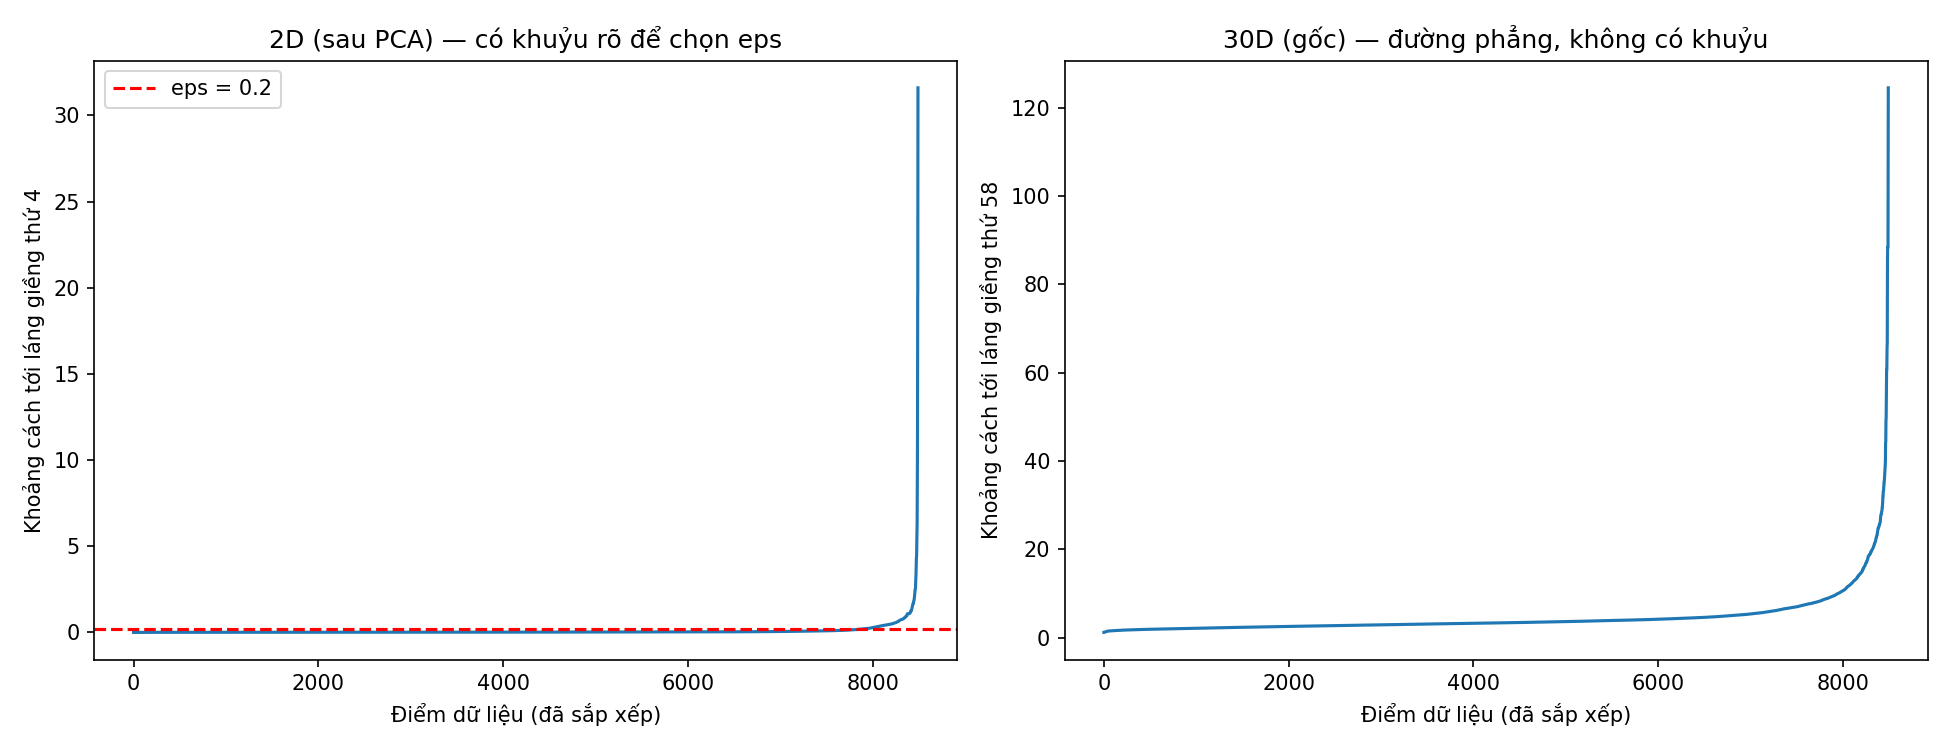
\includegraphics[width=0.72\textwidth]{k_distance.png}
  \end{center}
  \note{"Khi áp dụng DBSCAN vào thực tế, ta vướng hai rào cản: khối lượng dữ liệu khổng
  lồ và lời nguyền số chiều 30 chiều khiến khoảng cách mất ý nghĩa. Do đó chúng tôi
  lấy mẫu cân bằng, chuẩn hóa bằng RobustScaler để hạn chế nhiễu, rồi dùng PCA giảm
  xuống 2 chiều. Hình so sánh k-distance: ở 2D có khuỷu rõ để chọn eps, còn ở 30D đường
  phẳng --- chứng minh vì sao phải giảm chiều."}
\end{frame}

% =====================================================================
% Slide 5 — Kết quả Demo
% =====================================================================
\begin{frame}{Kết quả Demo: DBSCAN trên không gian 2D}
  \mellow
  \begin{columns}
    \begin{column}{0.62\textwidth}
      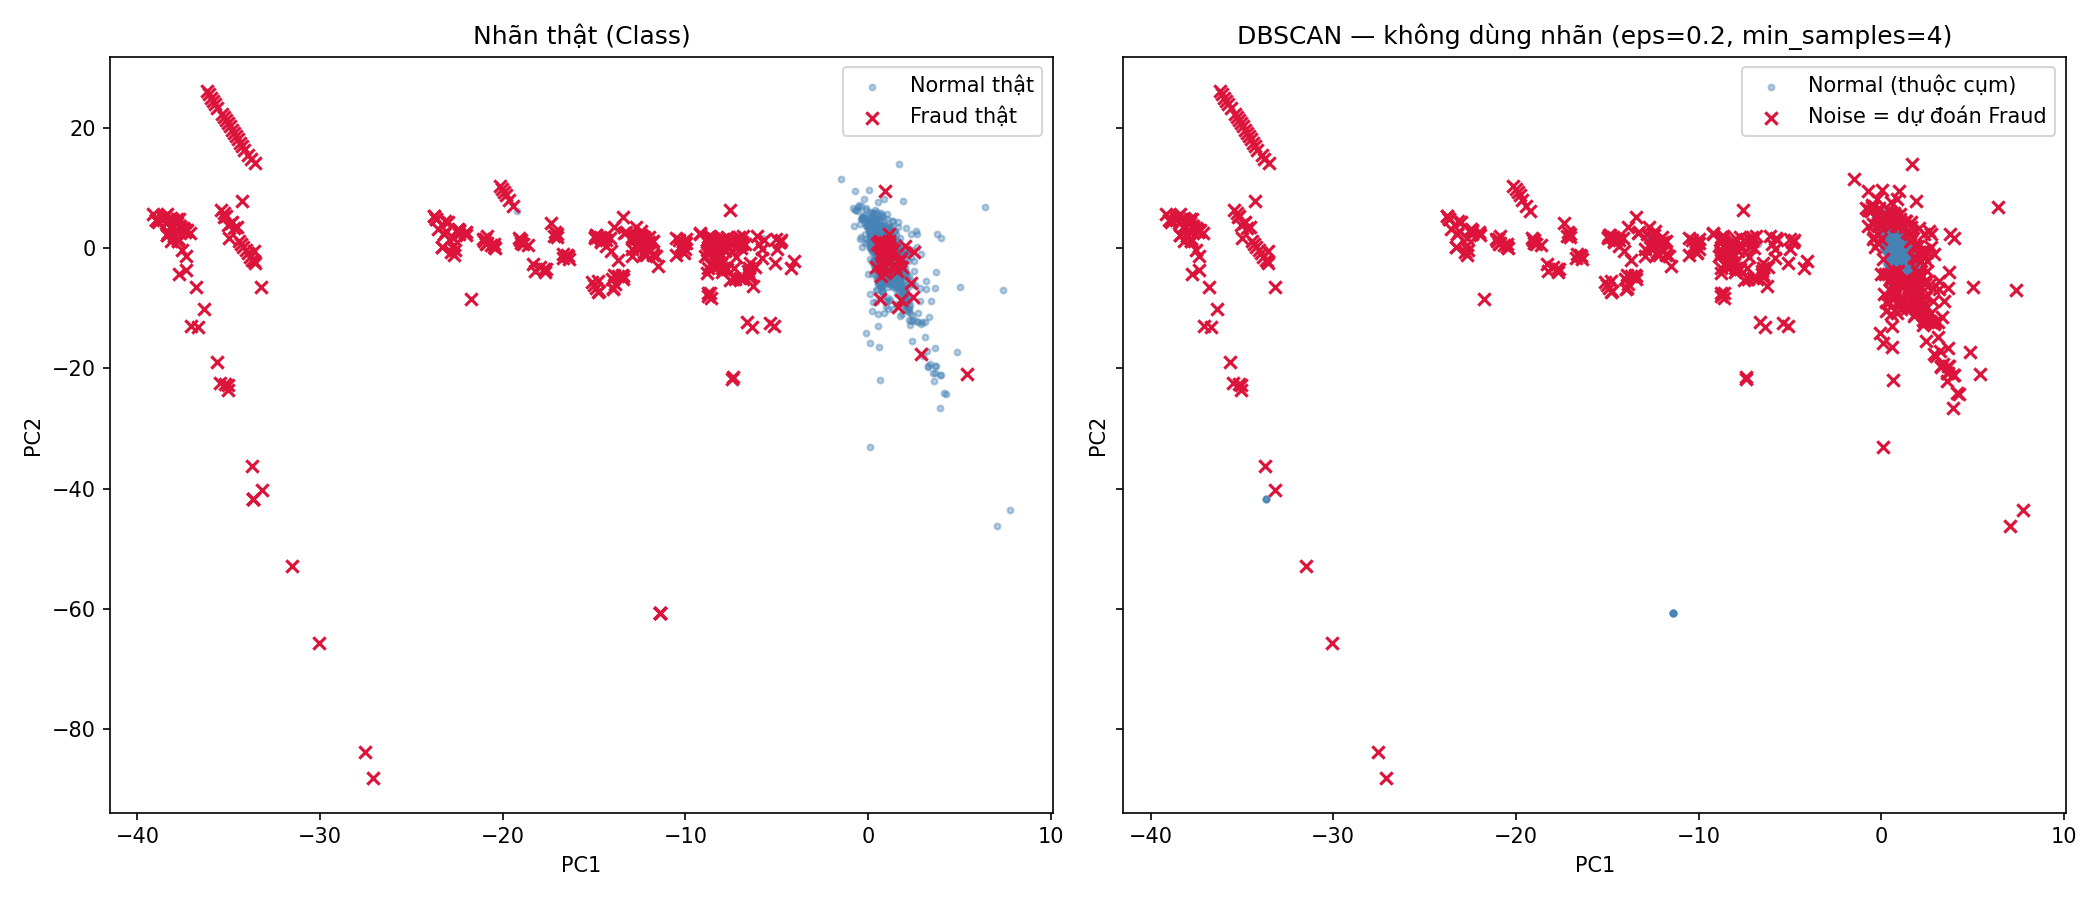
\includegraphics[width=\textwidth]{dbscan_fraud.png}
    \end{column}
    \begin{column}{0.38\textwidth}
      \begin{itemize}
        \item Cụm \textbf{xanh}: giao dịch bình thường
        \item Dấu \textbf{x đỏ}: Noise do DBSCAN phát hiện (ứng viên gian lận)
        \item Khoanh vùng thành công phần lớn điểm gian lận ở vùng biên, thưa thớt
      \end{itemize}
    \end{column}
  \end{columns}
  \begin{block}{Đánh giá nhanh (eps = 0,2)}
    Precision 0,62 \quad·\quad Recall 0,68 \quad·\quad AUPRC 0,44
  \end{block}
  \note{"Nhìn lên biểu đồ, các giao dịch bình thường quây tụ thành cụm xanh, còn các
  dấu thập đỏ chính là Noise do DBSCAN phát hiện. Thuật toán đã khoanh vùng và bắt được
  phần lớn điểm gian lận nằm ở vùng thưa thớt, chứng minh tính khả thi của học không
  giám sát: không cần nhãn vẫn bắt được 68\% gian lận."}
\end{frame}

% =====================================================================
% Slide 6 — Giới hạn & Hướng thay thế
% =====================================================================
\begin{frame}{Giới hạn của DBSCAN \& Hướng thay thế}
  \mellow
  \begin{block}{Nhược điểm}
    \begin{itemize}
      \item False Positive (báo động giả) với giao dịch số tiền lớn của khách VIP
      \item Không trả về xác suất rủi ro (Risk Score) dạng liên tục
      \item Không phù hợp hệ thống Real-time hiệu năng cao
    \end{itemize}
  \end{block}
  \begin{block}{Giải pháp thay thế}
    \begin{itemize}
      \item \textbf{Isolation Forest}: hiệu quả với không gian cao chiều
      \item \textbf{XGBoost}: khi đã có đủ nhãn lịch sử
    \end{itemize}
  \end{block}
  \note{"Tuy nhiên DBSCAN có điểm yếu cố hữu: báo động giả với khách VIP chi tiêu lớn
  bất thường, và không cung cấp điểm rủi ro liên tục 0--100\%. Vì vậy trong hệ thống
  thực tế cần real-time và xếp hạng mức độ nguy hiểm, ta nên chuyển sang Isolation
  Forest hoặc mô hình có giám sát XGBoost."}
\end{frame}

\end{document}
